\section{Conclusion and Outlook}%
\label{sec:result_discussion}

The results of the search for SM~\HH and resonant \HH production in the
\bbtautau channel are discussed in the following. The search is primarily
limited by uncertainties originating from the finite size of the \pp~collision
dataset collected during Run~2 of the LHC, which have the largest impact on the
extracted signal strengths and cross sections. Systematic uncertainties are
small and only relevant for searches for low-mass resonances. As a result, the
sensitivity of this search greatly benefits from the increase in integrated
luminosity compared to earlier searches
(cf.~\Cref{seq:experimental_status}). Improvements in the analysis, mostly in
the reconstruction and selection of physics objects, further increase the
sensitivity to resonant and non-resonant \HH production. Finally, this chapter
is concluded with an outlook on the expected sensitivity of searches for Higgs
boson pair production at the end of the HL-LHC.
% Prospects of these searches are studied by the ATLAS collaboration
% in~\cite{ATL-PHYS-PUB-2021-044,ATL-PHYS-PUB-2022-005} and are briefly
% discussed.

\subsection{Search for SM \HH Production}

To date, the SM~\HH search presented in this chapter has the highest expected
sensitivity to SM~\HH production of any single analysis channel. This is shown
in \Cref{fig:run2_hh_results}, which compares the upper limits on the SM~\HH
signal strength of searches conducted by the ATLAS and CMS collaborations. In
addition, the ATLAS and CMS collaborations performed statistical combinations of
the most relevant channels~(cf.~\Cref{fig:run2_hh_results}), yielding observed
(expected) upper limits on the SM~\HH signal strength of 2.4 and 3.4 (2.9 and
2.5), respectively~\cite{HDBS-2022-03,CMS-HIG-22-001}.
% the combination of the most sensitive channels yield observed (expected) upper
% limits on the SM~\HH signal strength of 2.4 and 3.4 (2.9 and 2.5) for the
% ATLAS and CMS collaboration, respectively~\cite{HDBS-2022-03,CMS-HIG-22-001}.
In general, similar results are obtained by both collaborations; however,
different analysis strategies are used in the \bbbb channels, which show the
largest difference between collaborations. While the ATLAS collaboration only
considers event topologies where the jet reconstruction can resolve all four
$b$-jets~\cite{ATLAS-CONF-2022-035}, the CMS collaboration also considers
boosted topologies in which the $b$-jet pairs are reconstructed as large-radius
jets~\cite{CMS-HIG-20-005,CMS-B2G-22-003}.

\begin{figure}[tbp]
  \centering

  \begin{subfigure}[b]{\textwidth}
    \centering

    \hspace{0.98em}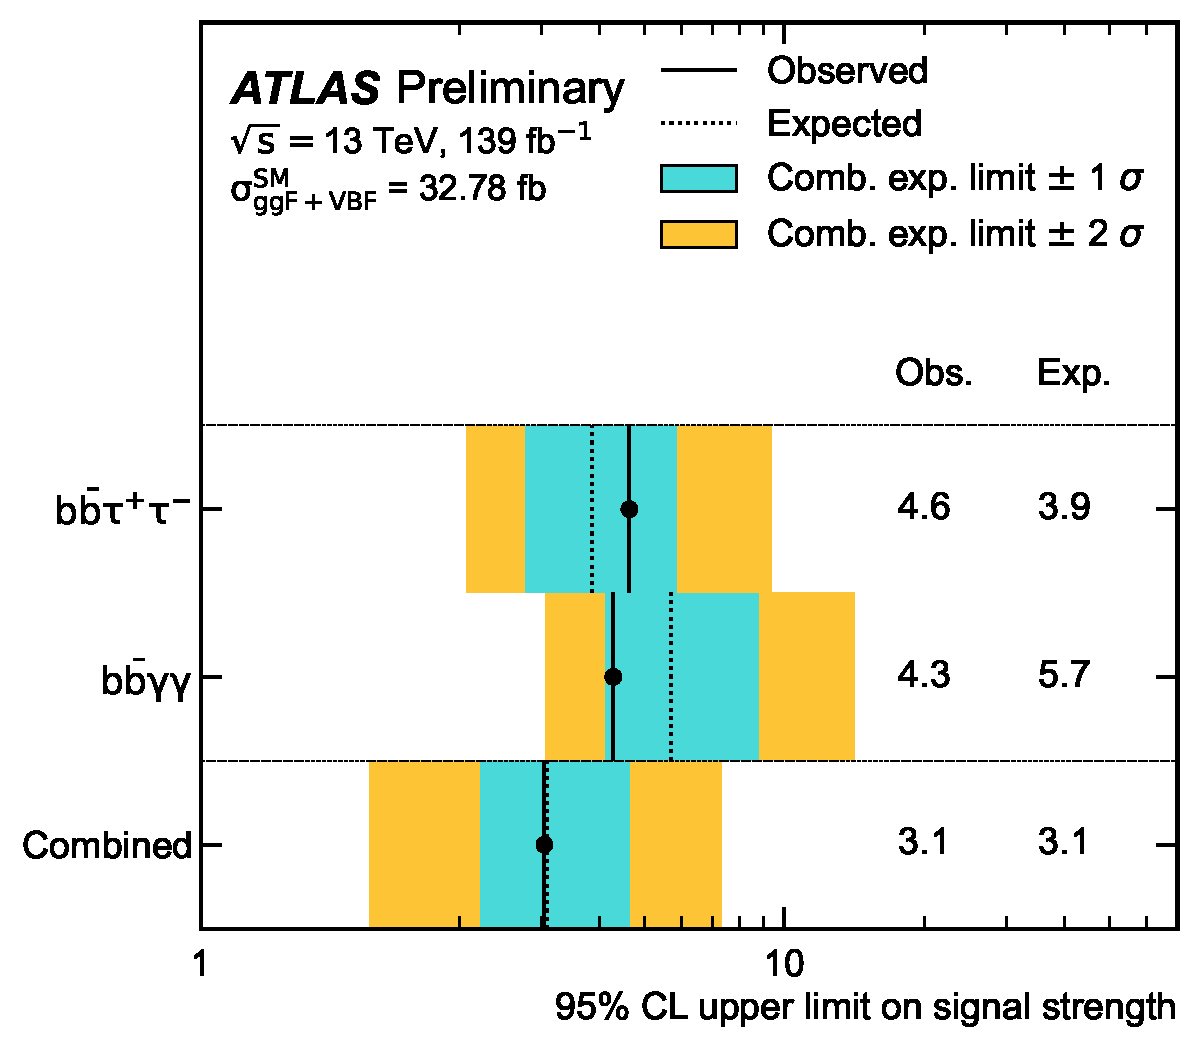
\includegraphics[width=0.585\textwidth]{discussion/results_139ifb}

    \subcaption{Results of SM~\HH searches by the ATLAS collaboration. The
      figure is taken from Ref.~\cite{HDBS-2022-03}.}%
    \label{fig:atlas_run2_139ifb}
  \end{subfigure}

  \vspace{12pt}

  \begin{subfigure}[b]{\textwidth}
    \centering

    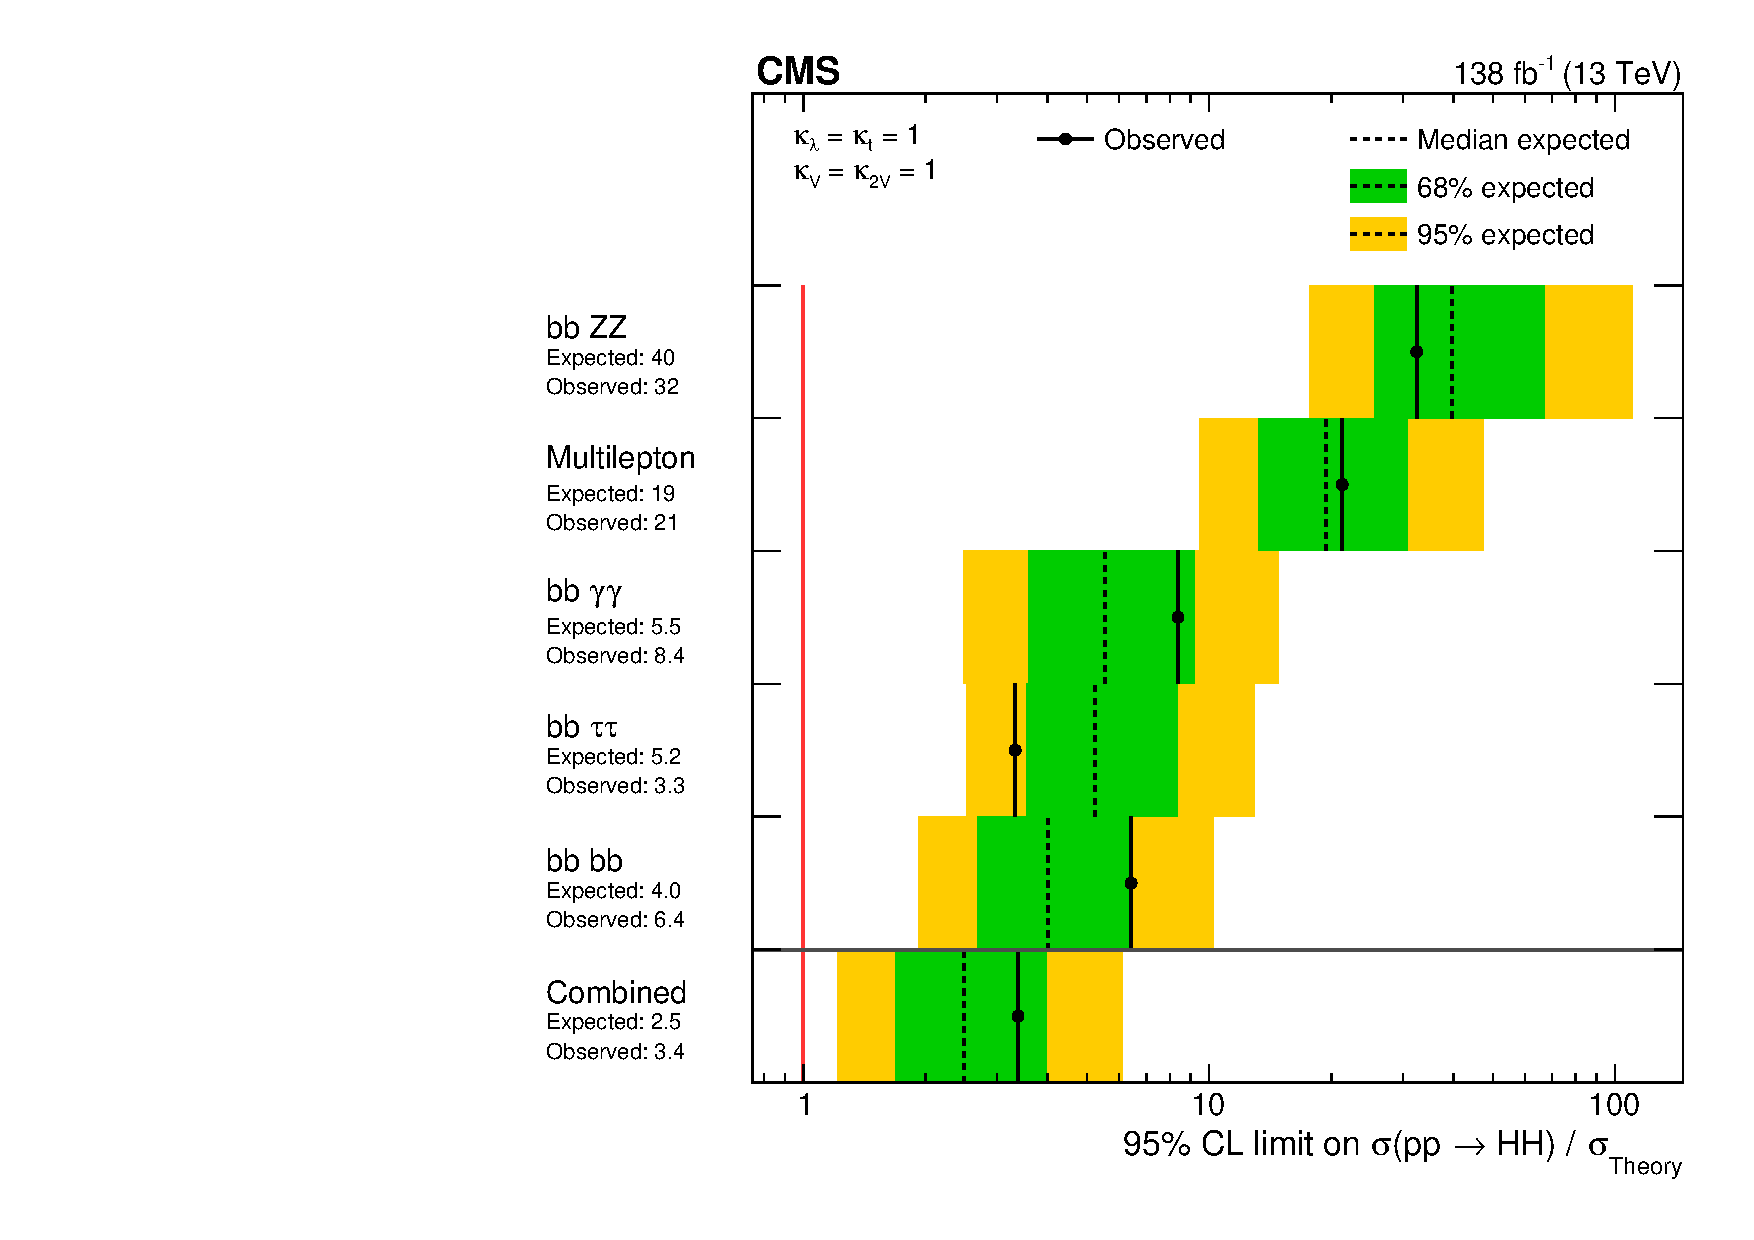
\includegraphics[width=0.611\textwidth]{discussion/cms_results_run2}

    \subcaption{Results of SM~\HH searches by the CMS collaboration. The
      multilepton channel targets $WWWW$, $WW\tau\tau$, and $\tau\tau\tau\tau$
      final states with two or more reconstructed $e$, $\mu$, or
      \tauhadvis~\cite{CMS-HIG-21-002}. The figure is taken
      from Ref.~\cite{CMS-HIG-22-001}.}%
    \label{fig:cms_run2_138ifb}
  \end{subfigure}

  \caption[Upper limits on the signal strength of SM~\HH production at
  \SI{95}{\percent}~CL by the ATLAS and CMS collaborations.]{Upper limits on the
    signal strength of SM~\HH production at \SI{95}{\percent}~CL by the
    ATLAS~(a) and CMS~(b) collaborations using \pp~collisions recorded during
    Run~2 of the LHC. The upper limits are shown for different analysis channels
    and their combination. The expected upper limits are derived assuming the
    absence of SM~\HH production.}%
  \label{fig:run2_hh_results}
\end{figure}

% This paragraph is weird given that CMS sees a different ordering of 'best
% channels'
%
% With the currently available dataset and experimental constraints (due to
% triggers, reconstruction, identification / isolation) of the ATLAS experiment
% for Run~2 of the LHC, the \bbtautau channel achieves a trade-off between the
% competing \bbyy and \bbbb channels regarding the search for SM \HH
% production. While the \bbyy channel provides access to events with low \mHH
% due to the ability to trigger on the signature of photons with low momentum
% thresholds (this is particularly advantageous when considering anomalous
% values of the Higgs boson self-couplings, cf.~REFERENCE) and a large
% background rejection due to the excellent $\gamma\gamma$ mass resolution, it
% is subject to the very small $\PHiggs \to \gamma\gamma$ branching ratio. In
% contrast, the largest fraction of SM \HH events are expected in the \bbbb
% final state, however, the measurement of SM \HH production in this channel is
% challenging due to the fully hadronic final state being subject to large
% multi-jet backgrounds and difficulties in selecting signal candidate events at
% trigger-level\footnote{There are also combinatorial difficulties in
% reconstructing $\PHiggs \to \bbbar$ candidates in the \bbbb channel where it
% can be ambiguous (particularly at low \mHH) how $b$-jets are paired into Higgs
% boson candidates. However, SM \HH production is produced at sufficiently high
% \mHH such that this is not really a huge issue.}. The \bbtautau final state,
% particularly in the \hadhad channel due to less prevalence of \ttbar
% backgrounds compared to the \lephad channel, is very sensitive to SM \HH
% production as signal events can be efficiently selected using \tauhadvis
% triggers due to their hard \mHH spectrum. The presence of \tauhadvis (and
% electrons / muons) provides large rejection power against multi-jet
% backgrounds compared to the \bbbb channel. Moreover, the fraction of SM \HH
% events decaying into \bbtautau final states is significantly larger than that
% of \bbyy.

The upper limit on the SM~\HH signal strength determined in this chapter is
compared to the previous result of the ATLAS collaboration in the \bbtautau
channel (cf.~\Cref{seq:experimental_status}). Using \SI{36.1}{\per\femto\barn}
of \pp~collisions recorded at the beginning of Run~2, the ATLAS collaboration
obtained an expected upper limit on the signal strength of SM~\HH production via
\ggF of 14.8 for the combination of the \lephad and \hadhad
channels~\cite{HIGG-2016-16-witherratum}. With the \SI{139}{\per\femto\barn}
\pp~collision dataset, an expected upper limit of 3.9 is set on the signal
strength of SM~\HH production via \ggF and VBF. The improvement in the upper
limit exceeds the expectation from a naive extrapolation of the previous result
to an integrated luminosity of \SI{139}{\per\femto\barn}, which would yield an
expected upper limit of approximately 7.\footnote{Neglecting systematic
  uncertainties and assuming that the upper limit scales with the integrated
  luminosity as a Poisson counting experiment.} This is primarily for two
reasons:
\begin{itemize}

\item The signal acceptance in the \hadhad (\lephad) channel improved by a
  factor of about 2 (1.5) due to improvements in $b$-tagging, \tauhadvis
  reconstruction, and \tauhadvis identification. At the same time, the rates of
  backgrounds with mistagged jets or \faketauhadvis remain comparable to the
  earlier analysis.

\item More events populate the signal-like region of the MVA discriminants as
  the integrated luminosity increases. This affects the re-binning algorithm due
  to the constraints on the minimum expected number of background events imposed
  on all bins. Consequently, as the integrated luminosity increases, the
  re-binning algorithm yields narrower bins in the high MVA score regions. Since
  the signal-to-background ratio increases quickly at high MVA score, narrower
  bins allow for better exploitation of the distinct signature of SM~\HH
  production.
  % Probably should put a number on this?

\end{itemize}

An outlook on future searches for Higgs boson pair production is provided by
extrapolations of the Run~2 results to the conditions after HL-LHC
data-taking. The SM~\HH search presented in this chapter was extrapolated by the
ATLAS collaboration to an integrated luminosity of \SI{3000}{\per\femto\barn}
and $\sqrt{s} = \SI{14}{\TeV}$ in Ref.~\cite{ATL-PHYS-PUB-2021-044}. This
extrapolation is conducted under the assumption that the performance of the
ATLAS detector can be maintained at the level of the Run~2 performance in spite
of the increase in instantaneous luminosity at the HL-LHC. In addition, the
evolution of systematic uncertainties follows the recommendations in
Ref.~\cite{ATL-PHYS-PUB-2019-005}. Given these assumptions the extrapolation of
the search for SM~\HH production in the \bbtautau channel yields an expected
discovery significance of $2.8 \sigma$ under the SM
hypothesis~\cite{ATL-PHYS-PUB-2021-044}.
% Thus evidence for non-resonant SM \HH production for a search in solely in the
% \bbtautau channel is in reach provided some improvements can be made.
A similar extrapolation was performed in the \bbyy channel resulting in an
expected significance of $2.2 \sigma$~\cite{ATL-PHYS-PUB-2022-001}. Furthermore,
the prospects of combining the \bbtautau and \bbyy channels at the end of the
HL-LHC were investigated in Ref.~\cite{ATL-PHYS-PUB-2022-005} suggesting that
evidence for SM~\HH production can be obtained with an expected significance of
$3.2 \sigma$ for the combination of both channels. Exceeding the discovery
threshold of $5 \sigma$ at the end of the HL-LHC is realistic but would require
the combination of the most sensitive channels of the ATLAS and CMS
collaborations as well as substantial improvements in the individual search
channels.

% Extrapolations under similar assumptions were performed for the \bbyy search
% channel yielding a significance of
% $2.2\,\sigma$~\cite{ATL-PHYS-PUB-2022-001}. Further, the prospects of
% combining the \bbtautau and \bbyy searches at the end of the HL-LHC were
% investigated in Ref.~\cite{ATL-PHYS-PUB-2022-005} suggesting that evidence for
% SM \HH production can be obtained with a discovery significance of
% $3.2\,\sigma$ for the combination of both channels. A discovery ($5\,\sigma$)
% of SM \HH production at the end of the HL-LHC is realistic but will likely
% require the combination of the most sensitive channels across both the ATLAS
% and CMS\todo{and substantial improvements in the invidual analyses.}
% collaborations.\footnote{For prospects of SM \HH searches by the CMS
% collaboration see Refs.~\cite{CMS-PAS-FTR-18-019} and
% \cite{CMS-PAS-FTR-21-004} from the beginning and the end of Run~2,
% respectively.}
% %   https://cms-results.web.cern.ch/cms-results/public-results/preliminary-results/FTR/index.html

% \todo[inline]{Check
% \url{https://cds.cern.ch/record/2805993/files/ATL-PHYS-PUB-2022-018.pdf} for
% ATLAS+CMS combination discovery significance. And this:
% \url{https://cds.cern.ch/record/2703572/files/94-87-PB.pdf} (4 sigma).  }

%   \todo[inline]{\url{https://twiki.cern.ch/twiki/bin/view/CMSPublic/SummaryResultsHIG}}

\subsection{Search for Resonant \HH Production}

The sensitivity of the \bbtautau channel to Higgs boson pair production via
scalar, narrow-width resonances is complementary to the \bbyy and \bbbb
channels. This is illustrated in \Cref{fig:resonant_hh_limits}, which compares
the upper limits on $\sigma(\pp \to X \to \HH)$ set by the ATLAS collaboration
in the \bbbb, \bbyy, and \bbtautau channel. The \bbtautau channel provides the
highest expected sensitivity of the three channels for resonances in an
intermediate mass range from \SIrange{375}{800}{\GeV}. For
$\mX < \SI{375}{\GeV}$, the \bbyy channel yields the most stringent upper limits
due to its use of di-photon triggers and the excellent background rejection
based on the invariant di-photon mass.
% The \bbyy channel yields the most stringent upper limits for
% $\mX < \SI{375}{\GeV}$ due to its use of di-photon triggers and excellent
% background rejection based on the invariant di-photon mass.
The highest expected sensitivity to resonances with $\mX > \SI{800}{\GeV}$ is
provided by the \bbbb channel due to the large $H \to \bbbar$ branching ratio,
$b$-jet triggers becoming increasingly efficient at selecting events with large
\mHH, and the use of special techniques to reconstruct events with highly
boosted Higgs bosons for $\SI{900}{\GeV} \leq \mX \leq \SI{5}{\TeV}$.

\begin{figure}[htbp]
  \centering

  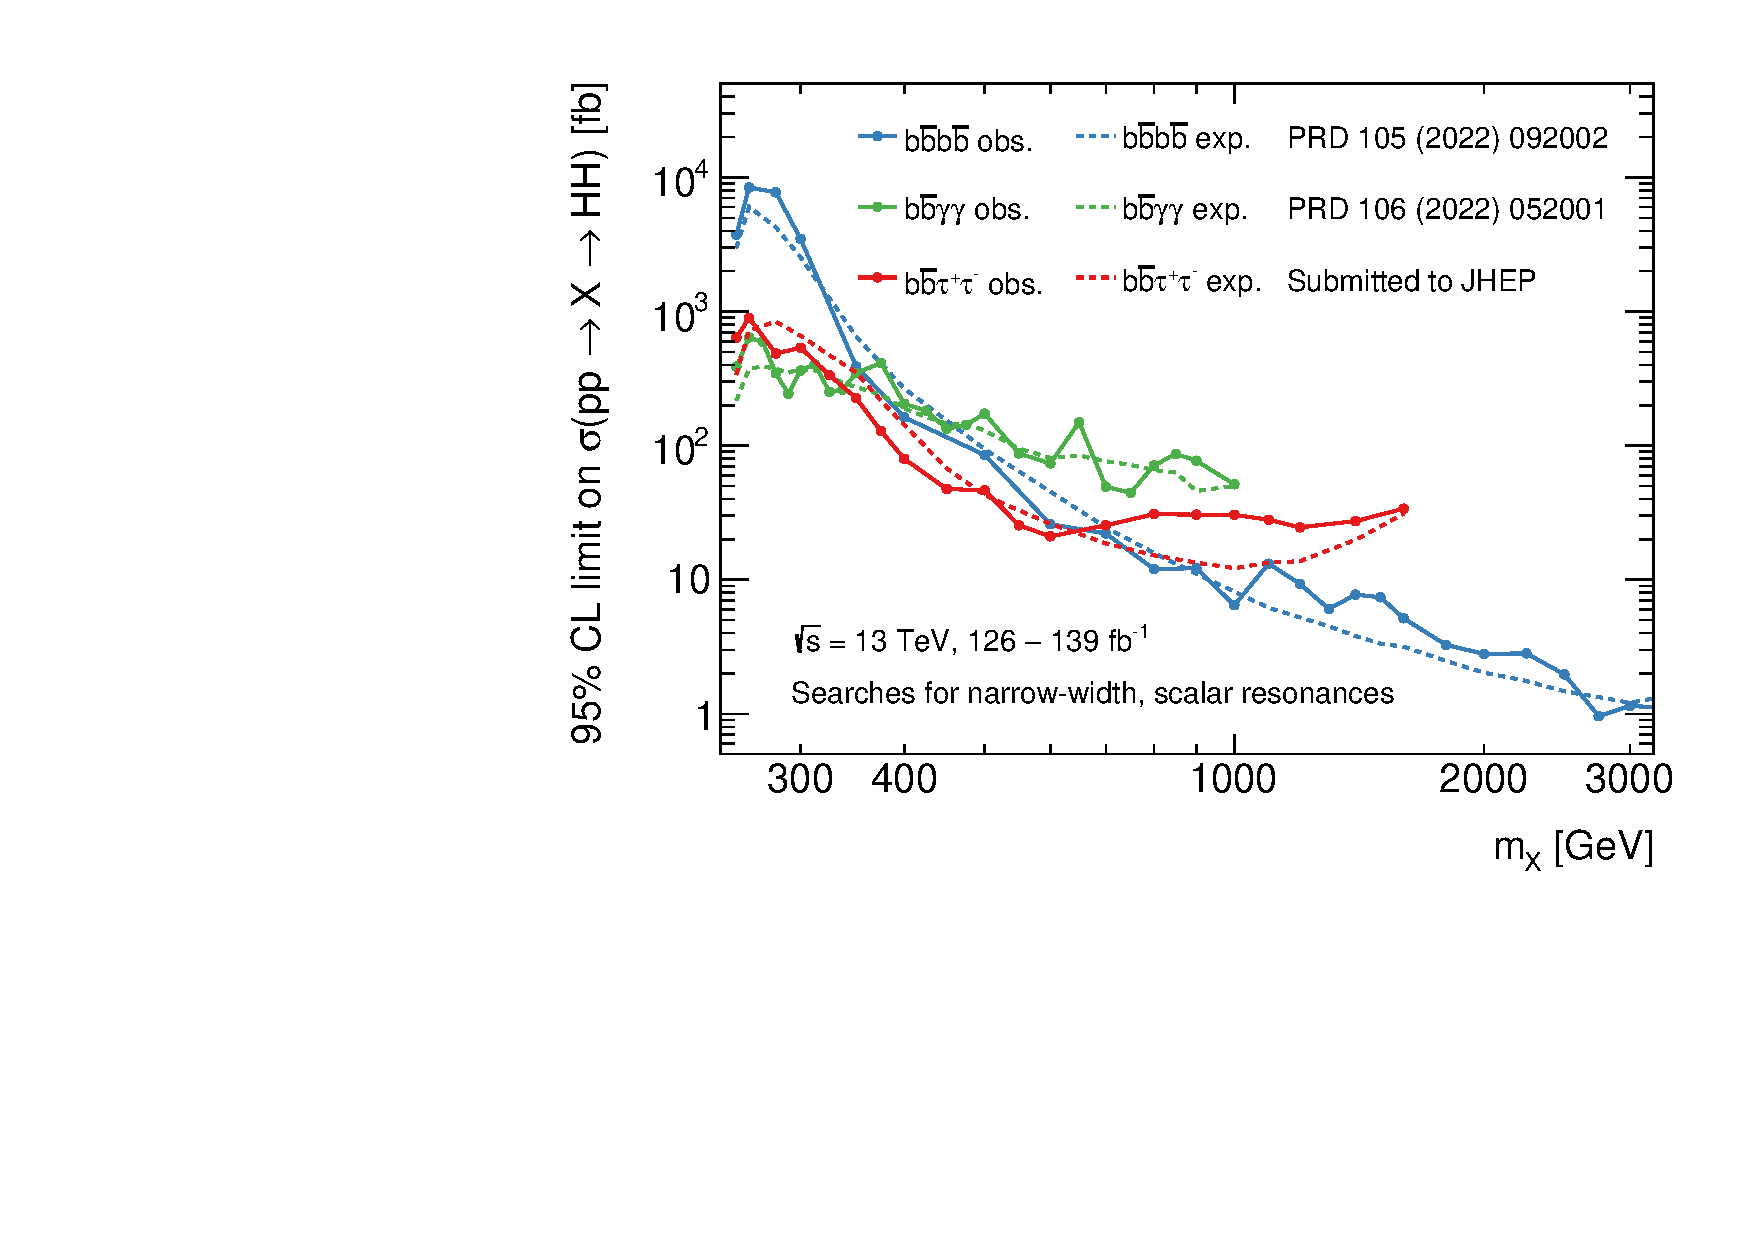
\includegraphics[width=0.65\textwidth]{discussion/atlas_comparison_resonant}

  \caption[Expected and observed upper limits on $\sigma(\pp \to X \to \HH)$ at
  \SI{95}{\percent}~CL.]{Expected (exp.) and observed (obs.) upper limits on
    $\sigma(\pp \to X \to \HH)$ at \SI{95}{\percent}~CL, where $X$ is a scalar,
    narrow-width resonance with mass \mX. Upper limits are shown separately for
    searches by the ATLAS collaboration in the
    \bbbb~\cite{HDBS-2018-41,hepdata.111124},
    \bbyy~\cite{HDBS-2018-34,hepdata.105864}, and \bbtautau
    channel~\cite{HDBS-2018-40}.}%
  \label{fig:resonant_hh_limits}
\end{figure}

The excess observed for $\mX = \SI{1000}{\GeV}$ in the \bbtautau channel with a
best-fit cross section of
$(17.4^{\hspace{0.25pt}+\hspace{0.25pt}7.5}_{-6.5})\valuesep\si{\femto\barn}$ is
compared to results of other searches. The search by the ATLAS collaboration in
the \bbbb channel yields an observed (expected) upper limit of
\SI{6.5}{\femto\barn} (\SI{8.1}{\femto\barn}) on $\sigma(\pp \to X \to \HH)$ at
$\mX = \SI{1000}{\GeV}$~\cite{HDBS-2018-41,hepdata.111124}. Therefore, the
best-fit cross section of the excess in the \bbtautau channel is excluded at
\SI{95}{\percent}~CL by the search in the \bbbb channel. In addition, the CMS
collaboration performed a search for resonant \HH production in boosted
topologies with \bbbar and one or two charged leptons (electrons or muons) in
Ref.~\cite{CMS-B2G-20-007}. This search provides similar sensitivity as the
ATLAS search in the \bbbb channel for $\mX \geq \SI{1}{\TeV}$ and yields
observed (expected) upper limits on $\sigma(\pp \to X \to \HH)$ of
\SI{4.8}{\femto\barn} (\SI{9.6}{\femto\barn}) for
$\mX = \SI{1000}{\GeV}$~\cite{CMS-B2G-20-007,hepdata.115024}. Similarly, this
search excludes the excess observed in the \bbtautau channel.

% https://cms-results.web.cern.ch/cms-results/public-results/publications/B2G-20-007/index.html

% CMS: X -> YH -> bbbb
% Excludes about 6 fb
% https://www.hepdata.net/record/ins2072383

% CMS Another comparison is provided by a search for resonant production of
% Higgs boson pairs with high momenta targeting final states with $b$-quarks and
% one or two light leptons (primarily $\bbbar W^+ W^-$ and
% $\bbbar \tau^+ \tau^-$) performed by the CMS collaboration in
% Ref.~\cite{CMS-B2G-20-007}. This analysis provides very stringent limits on
% the production of generic scalar resonances with narrow width and masses
% ranging from \SIrange{0.8}{4.5}{\TeV}. Observed (expected) upper limits on
% $\sigma(X \to \HH)$ are set at \SI{4.8}{\femto\barn} and \SI{3.4}{\femto\barn}
% (\SI{9.6}{\femto\barn} and \SI{7.1}{\femto\barn}) for resonance masses of
% \num{1000} and \SI{1100}{\GeV},
% respectively~\cite{CMS-B2G-20-007,hepdata.115024}. This analysis observes a
% deficit in data compared to the background prediction for masses close to
% \SI{1000}{\GeV}, suggesting that the features observed by the ATLAS
% collaboration are coincidental or from other sources.

% CMS resonant results:
%
% HH -> bbWW / bbtautau / bbZZ (boosted bb+l / ll final states)
% https://arxiv.org/pdf/2112.03161.pdf (published JHEP)
%                Obs.             Exp.
% 1000 GeV:      4.8 fb           9.6 fb
% 1100 GeV:      3.4 fb           7.1 fb
%
% - Too good to be true??? Probably fine
%
% HH -> 4b (boosted)
% https://cds.cern.ch/record/2777083/files/B2G-20-004-pas.pdf (preliminary)
%                Obs.             Exp.
% 1000 GeV:      28 fb            15 fb
% 1100 GeV:      9.9 fb           9.4 fb
%
% - Also an excess at 1 TeV (2 sigma ish)
% - None at 1.1 TeV

In conclusion, a search for resonant Higgs boson pair production in the
\bbtautau channel was presented. This search provides the best expected
sensitivity of ATLAS searches in the mass range from \SIrange{375}{800}{\GeV},
with upper limits on $\sigma(\pp \to X \to \HH)$ ranging from
\SIrange{130}{30}{\femto\barn} in this range. A broad excess is observed at
$\mX = \SI{1000}{\GeV}$ with a local (global) significance of $3.1\sigma$
($2.0\sigma$). The width of the excess is generally compatible with the
expectation of a real signal. However, after accounting for multiple hypothesis
testing, the excess was not found to be statistically significant. In addition,
other searches by the ATLAS and CMS collaborations do not support the observed
excess. Therefore, it is assumed that the excess originates from a statistical
fluctuation or a systematic issue, for example, a mismodelling of backgrounds.

% While the observed excess might have arisen from a statistical fluctuation of
% background events, it will be instructive for future iterations of this search
% to further scrutinise the background estimation methodology to rule out that
% these features are caused by a systematic mismodelling of the background. A
% candidate for inspection would be the \ZHF background, the largest background
% process in signal-like bins for high \mX discriminants in both the \hadhad and
% \lephad channels, for which the control region measurement of the \ZHF
% normalisation could be performed differentially to account for systematic
% shifts in the normalisation in certain regions of phase space. A variable to
% control for could be the transverse momentum of the $Z$ boson for which there
% are indications of systematic effects on the fitted normalisation (cf.\
% REFERENCE APPENDIX). Moreover, a comparison of reconstruction and
% identification efficiencies for highly collinear \tauhadvis between simulation
% and data would be further confirm that these topologies are not affected by
% miscalibrations of the efficiencies.

%%% Local Variables:
%%% mode: latex
%%% TeX-master: "../../phd_thesis"
%%% End:
